%% ===================================================================
%% PART I
%% ===================================================================
\part{Arithmetic origin and geometric foundations}

\section{Introduction: from arithmetic occurrences to geometry}\label{sec:intro}

\subsection{The question}

In the nest arithmetic of the UNNS Substrate, a pair $(N,M)$ of positive integers has the \emph{value}
\begin{equation}\label{eq:value}
  x \;=\; M\,\frac{(N+1)^2}{N}.
\end{equation}
Different pairs can have the same value. A small example is $x=36$: the pairs $(1,9)$, $(2,8)$ and $(5,5)$ all satisfy \eqref{eq:value} with $x=36$, since $9\cdot 4/1=8\cdot 9/2=5\cdot 36/5=36$. We call each such pair an \emph{occurrence} of the value. Equality of values is therefore an arithmetic fact about numbers, while identity of occurrences is a finer fact about pairs. This paper is about the finite configuration formed by all occurrences of one value, and the question it answers is the following.

\begin{quote}
\emph{What geometric structure can be built on the exact arithmetic coordinates of the occurrences of a single value, and how does that structure change as the range of admissible occurrences grows?}
\end{quote}

The arithmetic part of the answer is short and exact (Section~\ref{sec:arith}). If $x=a/b$ in lowest terms and $\kappa=N+1$, the occurrences of $x$ are in bijection with the integers $\kappa\ge 2$ such that $\kappa^2\mid a$ and $\kappa\equiv 1 \pmod b$. Writing $\kappa$ in terms of the prime factorization of $a$ identifies these occurrences with the nonzero points of a congruence lattice inside a box of exponent vectors. When two primes are active the lattice is, after a positive diagonal change of coordinates, the \emph{modular lattice}
\[
  \Gamma_{d,s}\;=\;\{(i,j)\in\Z^2:\ j\equiv s\,i \pmod d\},\qquad \gcd(s,d)=1,
\]
and the occurrences of $x$ are its nonzero points in a box $[0,Q_1]\times[0,Q_2]$ (Section~\ref{sec:planar}).

The geometric part is a construction. Two occurrences are related by an exact multiplicative relation between their indices, and the minimal such relations are \emph{Graver vectors} of the lattice, that is, conformally minimal lattice vectors. Using only Graver vectors we attach to the occurrence points all parallelograms, segments and points that they span (Section~\ref{sec:cells}). The resulting compact set $U_Q$ is the \emph{realized union}. It lies inside the convex hull $H_Q$ of the occurrence points. The paper determines when, and how, $U_Q$ fills $H_Q$.

\subsection{Terminology: arithmetic occurrence geometry}\label{sec:terminology}

We use the term \emph{arithmetic occurrence geometry} for the study of distinct arithmetic occurrences of a common numerical value, their exact coordinate relationships, and geometric structures explicitly constructed upon those relationships. In the UNNS framework such occurrences are represented by finite arithmetic fibres obtained from prime-exponent coordinates and congruence relations (Section~\ref{sec:arith}); the resulting point configurations are the arithmetic foundation for constructions involving Graver generators, admissible cells, convex hulls, topological invariants and embedding properties. The occurrence coordinates are determined by arithmetic. The geometric cell constructions are separately specified mathematical structures: arithmetic occurrence geometry thus distinguishes the intrinsic organization of the occurrences from the properties of a particular geometric realization. The formal definition is Definition~\ref{def:aog}, placed directly after the derivation of the fibre $F_x$. The term is a defined term of this work; the scope note at the end of Section~\ref{sec:lit} says what it does not mean.

The companion manuscript, Paper~B (a separate manuscript released together with this one), studies embedding obstructions in a binary $0/1$ specialisation of the same Graver-cell construction.

\subsection{Main results}

Throughout, $d\ge 2$ is an integer, $s$ is an integer unit modulo $d$, $t\equiv s^{-1}\pmod d$, and $Q=(Q_1,Q_2)$ is an integer box with $Q_1,Q_2\ge d$. We write $F_Q=(\Gamma_{d,s}\cap[0,Q_1]\times[0,Q_2])\setminus\{0\}$, $H_Q=\conv F_Q$ and $U_Q\subseteq H_Q$ for the realized union, all defined precisely in Section~\ref{sec:cells}. The \emph{exceptional box} is $Q_0=(d,d)$; we write $H_0$ and $U_0$ for $H_{Q_0}$ and $U_{Q_0}$.

\begin{theorem}[Occurrence-coordinate correspondence; Theorem~\ref{thm:occ}]
For a reduced rational $x=a/b>0$, the occurrences of $x$ are in bijection with $D(x)=\{\kappa\ge2:\kappa^2\mid a,\ \kappa\equiv1 \pmod b\}$, and $D(x)$ is in bijection with $F_x=(\Lambda_b\cap[0,q])\setminus\{0\}$, where $\Lambda_b$ is the kernel of the homomorphism $\Z^k\to(\Z/b)^\times$, $\alpha\mapsto\prod_i p_i^{\alpha_i}$. When two prime coordinates are active, $\Lambda_b$ is the image of $\Gamma_{d,s}$ under a positive diagonal map for suitable $d\ge1$ and $s$, and the box is $\bigl(\lfloor q_1/\lambda_1\rfloor,\lfloor q_2/\lambda_2\rfloor\bigr)$.
\end{theorem}

\begin{theorem}[Exact exceptional complement; Theorem~\ref{thm:exceptional}]
Let $d\ge5$, $2\le s\le d-2$, $\gcd(s,d)=1$. Then
\[
  H_0\setminus U_0=\interior T_1\sqcup\interior T_2,
\]
where $T_1,T_2$ are two explicit lattice triangles of area $d/2$ with a common vertex $(d,d)$. In particular $U_0$ has exactly two bounded complementary components and $\beta_1(U_0)=2$. For $s\equiv 1$ and $d\ge3$ the same identity holds (Proposition~\ref{prop:special-plus}); for $s\equiv-1$ the set $U_0$ is a fan graph with $\beta_1(U_0)=d$ (Proposition~\ref{prop:special-fan}).
\end{theorem}

\begin{theorem}[Hole filling; Proposition~\ref{prop:fill}]
For $d\ge3$, every unit $s$ and every box $Q\ge(d,d)$ with $Q\ne(d,d)$, the closed triangles $T_1,T_2$ lie in $U_Q$. Consequently $H_0\subseteq U_Q$ whenever the complement of $U_0$ in $H_0$ is exactly the two open triangles.
\end{theorem}

\begin{theorem}[Universal planar convex stabilization; Theorem~\ref{thm:universal}]\label{thm:intro-main}
For every $d\ge 2$, every unit $s$ modulo $d$, and every integer box $Q$ with $Q_1,Q_2\ge d$ and $Q\ne(d,d)$,
\[
  \boxed{\,U_{d,s,Q}=\conv\bigl(F_{d,s,Q}\bigr).\,}
\]
\end{theorem}

\begin{corollary}[Actual fibres; Corollary~\ref{cor:actual}]
Let $x=a/b$ have two active prime coordinates with $d\ge2$, $q_i\ge o_i$ for $i=1,2$ and $(\lfloor q_1/\lambda_1\rfloor,\lfloor q_2/\lambda_2\rfloor)\neq(d,d)$. Then the realized Graver-cell union of the occurrence fibre of $x$ equals its convex hull, and is contractible. The excluded case $\lfloor q_i/\lambda_i\rfloor=d$ is an arithmetic plateau $o_i\le q_i\le o_i+\lambda_i-1$, and there the union has exactly the topology described by the exceptional complement theorem.
\end{corollary}

For the pair of values $x_0=5^{10}3^{10}/11$ and $x_1=5^{12}3^{10}/11$ the first lies on the exceptional plateau and has seven occurrences with two holes; the second has eight occurrences and a convex realized union (Section~\ref{sec:example}). Raising a single prime exponent from $10$ to $12$ therefore changes the realized geometry from a set with two bounded complementary components to a full convex polygon.

\subsection{Scope and what is not claimed}

The results of this paper are statements about a specific, explicitly defined construction. We emphasize the following limits.

\begin{enumerate}
\item The construction is planar: it concerns two active prime coordinates. Occurrence fibres with three or more active primes are not treated.
\item The topology of $U_Q$ is the topology of the \emph{realized} point set defined in Section~\ref{sec:cells}. It is not asserted to be the unique topology forced by occurrence arithmetic. The attachment of cells is a modelling choice, motivated by arithmetic, and Section~\ref{sec:topology} separates what is proved about $U_Q$ from what would be a statement about an abstract cell complex.
\item The theorems say nothing about relations between occurrences of \emph{different} values. A global organization of occurrence geometry across fibres is an open problem (Section~\ref{sec:open}).
\item The case $d=1$ (that is, $\Lambda_b$ equal to a rectangular lattice $\lambda_1\Z\times\lambda_2\Z$) is outside the stabilization theorem.
\item Finite computations appear in this paper only as clearly separated checks and illustrations (Section~\ref{sec:provenance}). No universal statement is proved by computation.
\end{enumerate}

\subsection{Strategy of the proof}

The proof of Theorem~\ref{thm:intro-main} is a case analysis whose pieces are of quite different character.

\begin{itemize}
\item \emph{Special classes $s\equiv\pm1$} (Section~\ref{sec:special-stab}). Here the Graver bases can be written down in full, the lattice fibres into parallel lines, and the hull is swept by explicit parallelograms layer by layer.
\item \emph{Large boxes, $\max(Q_1,Q_2)\ge2d$} (Section~\ref{sec:large}). Every vertical line through the box contains at least two lattice points, and one tiles the hull column by column with vertically stacked translates of $(0,d)$-cells, together with correction triangles and two boundary slivers.
\item \emph{Small nonspecial boxes} $Q=(d+u,d+v)$ with $0\le u,v<d$ (Sections~\ref{sec:exceptional}--\ref{sec:fill} and \ref{sec:pareto}--\ref{sec:cap}). The old hull $H_0$ is covered in two steps: an exact description of the uncovered part of $H_0$ in the exceptional box (two open triangles), followed by the observation that each triangle is covered by an explicit cell as soon as the box grows. The remaining \emph{cap} $H_Q\setminus H_0$ is covered by an explicit family of translates of boundary edges by $(-d,0)$ and $(0,-d)$, plus one cell at each end of the outer boundary chain. These end cells are chosen using an arithmetic inequality for Pareto-minimal lattice points (Lemma~\ref{lem:arith}), and the validity of all the cells rests on a boundary lemma (Lemma~\ref{lem:reflection}) saying that consecutive boundary lattice points of $H_Q$ differ by Graver vectors.
\end{itemize}

\subsection{Organization}

Part~I (Sections~\ref{sec:intro}--\ref{sec:cells}) derives the arithmetic coordinates, the planar normalization, and the cell construction. Part~II (Sections~\ref{sec:exceptional}--\ref{sec:fill}) treats the exceptional square, its topology, and hole filling. Part~III (Sections~\ref{sec:special-stab}--\ref{sec:main}) contains the constructive proof of stabilization. Part~IV (Sections~\ref{sec:example}--\ref{sec:lit}) discusses actual occurrence fibres, consequences, and the literature. Part~V (Sections~\ref{sec:provenance}--\ref{sec:open}) records provenance and verification and formulates open problems. The appendices hold detailed calculations; none of the main arguments is deferred to them in the sense of being omitted. Appendix~\ref{app:registry} lists each theorem of this paper together with its source identifier in the GEO-I release series.

\subsection{Notation and conventions}

Table~\ref{tab:notation} collects the symbols used throughout. Vectors in $\Z^2$ are written $g=(g_1,g_2)$, and
\[
  \cross(g,h)=g_1h_2-g_2h_1.
\]
All homology groups have rational coefficients unless stated otherwise. For a set $S\subset\R^2$ we write $\conv S$, $\interior S$ and $\partial S$ for convex hull, interior and boundary. A \emph{lattice triangle} or \emph{lattice parallelogram} is one whose vertices lie in $\Z^2$.

\begin{table}[ht]
\centering\small
\begin{tabular}{@{}p{4.6cm}p{10.4cm}@{}}
\toprule
Symbol & Meaning\\
\midrule
$x=a/b$ & reduced positive rational value; $\kappa=N+1$ the occurrence index\\
$D(x)$ & set of occurrence indices of $x$\\
$p_1,\dots,p_k$, $q_i=\lfloor v_{p_i}(a)/2\rfloor$ & primes of $a$ and their exponent bounds\\
$\Lambda_b$, $F_x$ & relation lattice and punctured fibre in exponent coordinates\\
$d,s,t$ & modulus, unit, $t\equiv s^{-1}\pmod d$; $a_s=d-s$, $c_t=d-t$ (written $a,c$ from \S\ref{sec:exceptional} on)\\
$\Gamma_{d,s}$ & modular lattice $\{(i,j):j\equiv si\ (d)\}$\\
$Q=(Q_1,Q_2)$, $Q_0=(d,d)$ & integer box; exceptional box\\
$F_Q$, $H_Q$, $U_Q$ & punctured fibre, its convex hull, realized union\\
$h\conf g$ & conformal order\\
$P(w;g,h)$ & Graver parallelogram\\
$A=(0,d)$, $B=(d,0)$, $C_0=(d,d)$ & distinguished points of the exceptional box\\
$P_i=(i,si\bmod d)$ & residue points, $1\le i<d$\\
$T_1,T_2$ & the two exceptional triangles\\
$\Omega$ & outer boundary chain from $B$ to $A$, labelled in $\{R,C,T\}$\\
$\cross(g,h)$ & $g_1h_2-g_2h_1$\\
\bottomrule
\end{tabular}
\caption{Symbols.}\label{tab:notation}
\end{table}

%% -------------------------------------------------------------------
\section{Exact arithmetic of distinct occurrences}\label{sec:arith}

\subsection{Occurrences and their indices}

\begin{definition}[Occurrence]\label{def:occurrence}
An \emph{occurrence} is an ordered pair $(N,M)$ of positive integers. Its \emph{value} is $x(N,M)=M(N+1)^2/N\in\Q_{>0}$. An occurrence of the rational number $x$ is an occurrence $(N,M)$ with $x(N,M)=x$.
\end{definition}

Two occurrences are \emph{equal} only if they are the same pair. Two different occurrences may have equal value. The adjective ``distinct'' in this paper always refers to the pairs.

For a reduced fraction $x=a/b$ with $\gcd(a,b)=1$ put $\kappa=N+1\ge2$. Then \eqref{eq:value} is equivalent to
\begin{equation}\label{eq:occ-eq}
  a(\kappa-1)=b\,M\,\kappa^2.
\end{equation}

\begin{proposition}[Exact occurrence indices]\label{prop:bij}
Let $x=a/b>0$ with $\gcd(a,b)=1$. The map $(N,M)\mapsto\kappa=N+1$ is a bijection from the set of occurrences of $x$ onto
\[
  D(x)=\{\kappa\in\Z_{\ge2}:\ \kappa^2\mid a,\ \kappa\equiv1\pmod b\}.
\]
The inverse is $\kappa\mapsto\bigl(\kappa-1,\ \tfrac{a}{\kappa^2}\cdot\tfrac{\kappa-1}{b}\bigr)$.
\end{proposition}
\begin{proof}
Let $(N,M)$ be an occurrence of $x$ and $\kappa=N+1$. Then $\kappa\ge2$ and \eqref{eq:occ-eq} holds. Because $\gcd(\kappa^2,\kappa-1)=1$ and $\kappa^2\mid a(\kappa-1)$, we get $\kappa^2\mid a$. Because $\gcd(a,b)=1$ and $b\mid a(\kappa-1)$, we get $b\mid\kappa-1$. So $\kappa\in D(x)$, and $M=\frac a{\kappa^2}\cdot\frac{\kappa-1}b$ is determined by $\kappa$; the map is injective.

Conversely, if $\kappa\in D(x)$ then $N=\kappa-1\ge1$ and $M=\frac a{\kappa^2}\cdot\frac{\kappa-1}b$ is a positive integer, since $\kappa^2\mid a$ and $b\mid\kappa-1$. Then $M(N+1)^2/N=\frac{a(\kappa-1)}{b\kappa^2}\cdot\frac{\kappa^2}{\kappa-1}=a/b$.
\end{proof}

This is a bijective description of the distinct occurrences of $x$, not an approximation to them. For $x=36=36/1$ it gives $D(36)=\{2,3,6\}$ and recovers the three pairs listed in Section~\ref{sec:intro}: $\kappa=2$ gives $(N,M)=(1,9)$, $\kappa=3$ gives $(2,8)$, $\kappa=6$ gives $(5,5)$.

\subsection{Prime-exponent coordinates}

Let $a=\prod_{i=1}^kp_i^{e_i}$ be the prime factorization, $e_i\ge1$, and put $q_i=\lfloor e_i/2\rfloor$ and $q=(q_1,\dots,q_k)$. Since $\gcd(a,b)=1$, every $p_i$ is invertible modulo $b$. Define
\[
  \chi_b:\Z^k\to(\Z/b\Z)^\times,\qquad \chi_b(\alpha)=\prod_{i=1}^kp_i^{\alpha_i}\bmod b,
\]
a group homomorphism, and
\[
  \Lambda_b=\ker\chi_b=\Bigl\{\alpha\in\Z^k:\ \prod_{i}p_i^{\alpha_i}\equiv1\pmod b\Bigr\}.
\]

\begin{lemma}[Lattice kernel]\label{lem:kernel}
$\Lambda_b$ is a sublattice of $\Z^k$ of finite index $|\chi_b(\Z^k)|$ dividing $\varphi(b)$. In particular it has full rank $k$. Moreover, if $o_i$ is the multiplicative order of $p_i$ modulo $b$, then $o_i\mathbf e_i\in\Lambda_b$.
\end{lemma}
\begin{proof}
A kernel of a homomorphism to a finite abelian group is a subgroup of finite index, and a finite-index subgroup of $\Z^k$ is a full-rank lattice. The index equals the size of the image, a subgroup of $(\Z/b)^\times$, so it divides $\varphi(b)$. The last assertion is the definition of $o_i$.
\end{proof}

\begin{theorem}[Occurrence-coordinate correspondence]\label{thm:occ}
Let $x=a/b$ be reduced, with $p_i,q_i,\Lambda_b$ as above. The map
\[
  \alpha\ \longmapsto\ \kappa(\alpha)=\prod_{i=1}^kp_i^{\alpha_i}
\]
is a bijection from the \emph{punctured fibre}
\[
  F_x=(\Lambda_b\cap[0,q])\setminus\{\mathbf0\}
\]
onto $D(x)$, and hence the occurrences of $x$ are in bijection with $F_x$ by $\alpha\mapsto\bigl(\kappa(\alpha)-1,\ \tfrac{a}{\kappa(\alpha)^2}\tfrac{\kappa(\alpha)-1}{b}\bigr)$.
\end{theorem}
\begin{proof}
Let $\kappa\in D(x)$. Since $\kappa^2\mid a$, every prime dividing $\kappa$ is some $p_i$, and $\kappa=\prod p_i^{\alpha_i}$ with $2\alpha_i\le e_i$, that is $0\le\alpha_i\le q_i$. By unique factorization $\alpha$ is determined by $\kappa$, and $\kappa\equiv1\pmod b$ says $\alpha\in\Lambda_b$. Since $\kappa\ge2$, $\alpha\ne\mathbf 0$. Conversely every $\alpha\in(\Lambda_b\cap[0,q])\setminus\{\mathbf0\}$ gives $\kappa(\alpha)\ge2$ with $\kappa^2\mid a$ and $\kappa\equiv1\pmod b$. Combine with Proposition~\ref{prop:bij}.
\end{proof}

\begin{definition}[Arithmetic occurrence fibre; arithmetic occurrence geometry]\label{def:aog}
For a reduced rational $x=a/b>0$, the \emph{arithmetic occurrence fibre} of $x$ is the finite set $F_x=(\Lambda_b\cap[0,q])\setminus\{\mathbf0\}$ of Theorem~\ref{thm:occ}, regarded together with its bijection to the occurrences of $x$. Its \emph{exact coordinate relationships} are the differences of its points, which are lattice vectors of $\Lambda_b$ (Section~\ref{sec:arith-meaning}). \emph{Arithmetic occurrence geometry} is the study of arithmetic occurrence fibres, of their exact coordinate relationships, and of geometric realizations explicitly constructed upon those relationships. A \emph{realization} is a specified construction (in this paper the Graver-cell construction of Section~\ref{sec:cells}, its realized union and convex hull); the fibre and its coordinate relations are determined by arithmetic alone, while every property of a realization (filling, topology, embedding) is a property of that particular construction.
\end{definition}

\begin{remark}[Reading of the definition]
The definition names objects already defined and proved to exist above; it adds no hypothesis and changes no statement of this paper. In particular it does not make the geometry a branch of the established field of arithmetic geometry, whose definitions it does not inherit.
\end{remark}

\begin{remark}[The deleted origin]\label{rem:origin}
The exponent vector $\mathbf0$ corresponds to $\kappa=1$, that is to $N=0$, which is not an occurrence. The origin lies in every lattice $\Lambda_b$ and in every box, so it must be deleted explicitly. This deletion is not cosmetic: it is the source of the exceptional behaviour of the box $Q=(d,d)$ studied in Part~II, and of several degenerate cases in the boundary lemma (Lemma~\ref{lem:reflection}).
\end{remark}

\begin{remark}[Inactive coordinates]
A prime with $q_i=0$ (that is $e_i=1$) forces $\alpha_i=0$ and can be suppressed. We call the coordinates with $q_i\ge1$ \emph{active}. Throughout the geometry we work with the active coordinates only; the lattice is then the intersection of $\Lambda_b$ with the active coordinate subspace, which is again a kernel of a homomorphism, and Lemma~\ref{lem:kernel} applies verbatim.
\end{remark}

\subsection{Arithmetic content of lattice vectors}\label{sec:arith-meaning}

Let $\alpha,\alpha'\in F_x$ be two occurrence coordinates, with indices $\kappa,\kappa'$. Then $\kappa'/\kappa=\prod_ip_i^{\alpha'_i-\alpha_i}\equiv1\pmod b$ in the sense of $\chi_b$, so $g=\alpha'-\alpha\in\Lambda_b$. Thus the difference of two occurrence coordinates is a lattice vector, and every lattice vector is such a difference when the box is large enough. Writing $g=g^+-g^-$ with $g^\pm\ge0$ having disjoint supports, the vector $g$ records the congruence
\[
  \prod_ip_i^{g^+_i}\ \equiv\ \prod_ip_i^{g^-_i}\pmod b
\]
between two coprime integers. If a lattice vector $h\ne0,g$ satisfies $h\conf g$ (Definition~\ref{def:conformal} below), then $g-h$ is also a nonzero lattice vector with $g-h\conf g$, and $g=h+(g-h)$ splits the relation of $g$ into the relations of $h$ and of $g-h$, which have the same sign pattern as $g$. A conformally minimal vector therefore records a \emph{primitive} multiplicative relation between the indices: one that cannot be split into two relations with the same signs. This is the sense in which Graver vectors are arithmetically natural; it motivates the construction below, but it does not by itself force the attachment of two-dimensional cells (Remark~\ref{rem:modelling}).

\subsection{Arithmetic equality versus occurrence identity}

The same exponent vector $\alpha$ gives different occurrences for different values: for $\alpha\in F_x\cap F_{x'}$ the pair $(N,M)$ has the same $N=\kappa(\alpha)-1$ but $M=\frac{a}{\kappa^2}\frac{\kappa-1}{b}$ depends on $a/b$. In particular the inclusion $F_x\subseteq F_{x'}$ of exponent fibres, which occurs for $x'=x\cdot p_1^{2}$ (when $b$ and the other exponents are unchanged), does \emph{not} identify the occurrences of $x$ with those of $x'$. We return to this in Section~\ref{sec:example}, where $x_0$ and $x_1$ have the same relation lattice and nested exponent fibres but disjoint sets of occurrence pairs. A complete treatment of how fibres of different values are related is an open problem (Question~\ref{q:global}).

%% -------------------------------------------------------------------
\section{Planar normalization and modular relation lattices}\label{sec:planar}

We now treat the case of exactly two active prime coordinates, $k=2$. Let $r_i=p_i\bmod b\in(\Z/b)^\times$ and let $o_i=\ord_b(p_i)$ denote the multiplicative order of $r_i$. Put
\[
  D_0=\langle r_1\rangle\cap\langle r_2\rangle\ \le(\Z/b)^\times,\qquad d=|D_0|,\qquad \lambda_i=o_i/d.
\]
The group $D_0$ is a subgroup of the cyclic group $\langle r_1\rangle$, hence cyclic, and $d$ divides both $o_1$ and $o_2$ so that $\lambda_1,\lambda_2$ are positive integers.

\begin{proposition}[Planar normalization]\label{prop:norm}
Let $g_i=r_i^{\lambda_i}$. Then $g_1$ and $g_2$ each generate $D_0$.
\begin{enumerate}
\item If $\alpha_1,\alpha_2\in\Z$ satisfy $r_1^{\alpha_1}r_2^{\alpha_2}=1$ then $\lambda_i\mid\alpha_i$ ($i=1,2$).
\item If $d=1$ then $\Lambda_b=\lambda_1\Z\times\lambda_2\Z$.
\item If $d\ge2$ there is a unit $s$ modulo $d$, uniquely determined modulo $d$, such that $g_1=g_2^{-s}$. With this $s$,
\[
  \Lambda_b=\{(\lambda_1i,\lambda_2j):\ (i,j)\in\Gamma_{d,s}\},\qquad \Gamma_{d,s}=\{(i,j)\in\Z^2:\ j\equiv si\ (\mathrm{mod}\ d)\}.
\]
\end{enumerate}
\end{proposition}
\begin{proof}
The cyclic group $\langle r_i\rangle$ of order $o_i$ has a unique subgroup of order $d$, namely $\langle r_i^{o_i/d}\rangle=\langle g_i\rangle$. Both $\langle g_1\rangle$ and $\langle g_2\rangle$ are subgroups of order $d$ of $D_0$, and $D_0$ is cyclic of order $d$; hence $\langle g_1\rangle=D_0=\langle g_2\rangle$.

(1) If $r_1^{\alpha_1}r_2^{\alpha_2}=1$ then $r_1^{\alpha_1}=r_2^{-\alpha_2}\in\langle r_1\rangle\cap\langle r_2\rangle=D_0=\langle r_1^{\lambda_1}\rangle$. Since $r_1^{\alpha_1}\in\langle r_1^{\lambda_1}\rangle$ happens exactly when $\lambda_1\mid\alpha_1$ (using $\lambda_1\mid o_1$), we get $\lambda_1\mid\alpha_1$. Likewise $\lambda_2\mid\alpha_2$.

(2) and (3). By (1), every $\alpha\in\Lambda_b$ has the form $(\lambda_1i,\lambda_2j)$ and the defining condition becomes $g_1^ig_2^j=1$. For $d=1$ the group $D_0$ is trivial and the condition is empty, giving (2). For $d\ge2$, $g_1$ and $g_2$ are two generators of a cyclic group of order $d$, so $g_1=g_2^{\sigma}$ for a unit $\sigma$ modulo $d$, unique modulo $d$. Then $g_1^ig_2^j=g_2^{\sigma i+j}$, which is $1$ if and only if $j\equiv-\sigma i\pmod d$. Put $s\equiv-\sigma$.
\end{proof}

Let $L(i,j)=(\lambda_1i,\lambda_2j)$. The proposition says $\Lambda_b=L(\Gamma_{d,s})$ when $d\ge2$. The box constraint $0\le\alpha_i\le q_i$ translates into
\[
  0\le i\le Q_1:=\lfloor q_1/\lambda_1\rfloor,\qquad 0\le j\le Q_2:=\lfloor q_2/\lambda_2\rfloor,
\]
so that
\begin{equation}\label{eq:FxL}
  F_x=L\bigl(F_{d,s,Q}\bigr),\qquad F_{d,s,Q}=\bigl(\Gamma_{d,s}\cap[0,Q_1]\times[0,Q_2]\bigr)\setminus\{0\}.
\end{equation}

\begin{proposition}[Transfer]\label{prop:transfer}
The linear isomorphism $L$ of $\R^2$ maps $\Gamma_{d,s}$ onto $\Lambda_b$, preserves the conformal order in the sense that $h\conf g\iff Lh\conf Lg$, maps Graver vectors of $\Gamma_{d,s}$ to Graver vectors of $\Lambda_b$, convex hulls to convex hulls, and Graver parallelograms to Graver parallelograms. Consequently the realized Graver-cell union of the actual fibre $F_x\subset\Lambda_b$ is $L(U_{d,s,Q})$, and every topological statement about $U_{d,s,Q}$ holds for the actual fibre.
\end{proposition}
\begin{proof}
$L$ is linear and diagonal with positive entries, so $(Lh)_i(Lg)_i=\lambda_i^2h_ig_i$ has the same sign as $h_ig_i$, and $|(Lh)_i|\le|(Lg)_i|\iff|h_i|\le|g_i|$. Since $L$ is a bijection of $\Gamma_{d,s}$ onto $\Lambda_b$, minimality of $g$ in $\Gamma_{d,s}\setminus\{0\}$ is equivalent to minimality of $Lg$ in $\Lambda_b\setminus\{0\}$. The remaining assertions follow because an invertible linear map takes the convex hull of a set to the convex hull of its image and takes $P(w;g,h)$ to $P(Lw;Lg,Lh)$, with corners in $L(F_Q)=F_x$ exactly when the original corners are in $F_Q$ by \eqref{eq:FxL}.
\end{proof}

The case $d=1$ gives the rectangular lattice $\lambda_1\Z\times\lambda_2\Z$, for which every lattice point of the box is a fibre point and the Graver vectors are the scaled coordinate vectors; it is outside the stabilization theorem proved here (Remark~\ref{rem:d1}).

\subsection{Which normalized instances occur}

\begin{corollary}[Plateau of the exceptional box]\label{cor:plateau}
In the normalization above ($d\ge 2$), $\lfloor q_i/\lambda_i\rfloor= d$ if and only if $o_i\le q_i\le o_i+\lambda_i-1$. The normalized box satisfies $Q_i\ge d$ if and only if $q_i\ge o_i$.
\end{corollary}
\begin{proof}
$\lfloor q_i/\lambda_i\rfloor\ge d\iff q_i\ge d\lambda_i=o_i$ and $\lfloor q_i/\lambda_i\rfloor\le d\iff q_i<(d+1)\lambda_i=o_i+\lambda_i$.
\end{proof}

The proposition and its corollary identify the actual fibres to which the normalized theory applies. We distinguish two questions.

\begin{enumerate}
\item \emph{Reduction}: every actual planar fibre with $d\ge2$ is, via $L$, a normalized fibre $F_{d,s,Q}$ (Proposition~\ref{prop:norm}). This is a proved fact about every such value.
\item \emph{Realization}: conversely, is every normalized instance $(d,s,Q)$ the image of an actual value? The following proposition shows that it is, by an argument that uses Dirichlet's theorem on primes in arithmetic progressions in an essential way.
\end{enumerate}

\begin{proposition}[Realizability of normalized instances]\label{prop:realize}
For every integer $d\ge2$, every unit $s$ modulo $d$ and every pair $(Q_1,Q_2)$ of positive integers there exist primes $b,p_1,p_2$ with $p_1\ne p_2$, $p_i\neq b$, such that for $x=p_1^{2Q_1}p_2^{2Q_2}/b$ one has $\lambda_1=\lambda_2=1$ and the normalized parameters of Proposition~\ref{prop:norm} are exactly $(d,s,Q)$.
\end{proposition}
\begin{proof}
Choose a prime $b\equiv1\pmod d$ (Dirichlet's theorem; for the residue class $1$ this is elementary). The group $(\Z/b)^\times$ is cyclic of order $b-1$, so it has an element $h$ of order exactly $d$. Let $t\equiv s^{-1}\pmod d$ and $\tau\equiv-t\pmod d$, a unit. By Dirichlet's theorem choose distinct primes $p_1\equiv h$ and $p_2\equiv h^\tau\pmod b$, both different from $b$. Then $r_1=h$ and $r_2=h^\tau$ both generate $\langle h\rangle$, so $D_0=\langle h\rangle$, $d=|D_0|$, $o_1=o_2=d$, $\lambda_1=\lambda_2=1$. Moreover $g_1=h=(h^\tau)^{\tau^{-1}}=g_2^{\tau^{-1}}$; now $\tau^{-1}\equiv-s$, so $g_1=g_2^{-s}$, which means that the unit of Proposition~\ref{prop:norm}(3) is $s$. The exponent bounds of $x=p_1^{2Q_1}p_2^{2Q_2}/b$ are $q_i=Q_i$.
\end{proof}

\begin{remark}\label{rem:realize-status}
Proposition~\ref{prop:realize} is not part of the GEO-I release record; it is a short observation written for this manuscript, and it has been tested by a finite computation (Section~\ref{sec:provenance}) in addition to the proof above. None of the main theorems depends on it. Its role is to show that the study of the normalized family $\{\Gamma_{d,s}\}$ is not a study of auxiliary objects: each member, in each box, is the occurrence fibre of an explicit rational number. The primes $b,p_1,p_2$ are chosen depending on $(d,s)$; the proposition makes no claim about a prescribed pair of primes such as $(5,3)$ (for which $b=11$ gives $(d,s)=(5,2)$, Section~\ref{sec:example}).
\end{remark}

\begin{remark}[Normalized family in its own right]
The normalized family $\Gamma_{d,s}$ is also a mathematical object independent of arithmetic: Parts~II and III prove theorems about it for all $d\ge2$ and all units $s$, whether or not a given instance is considered together with a particular value. We do so because the statements are cleaner and because the transfer (Proposition~\ref{prop:transfer}) is exact.
\end{remark}

\begin{remark}[The case $d=1$]\label{rem:d1}
When $D_0$ is trivial, the relation lattice is rectangular and the occurrence fibre is the full set of lattice points $(\lambda_1i,\lambda_2j)$, $(i,j)\ne0$, of a box. For example $x=36$ has $b=1$, $\Lambda_1=\Z^2$ for the primes $2,3$, and $F_{36}=\{(1,0),(0,1),(1,1)\}$. The cell construction is trivial in this case (all of $H_Q$ is spanned by coordinate parallelograms, if the box has both sides at least $2$) and gives no exceptional square. We do not discuss it further.
\end{remark}

\begin{figure}[ht]
\centering
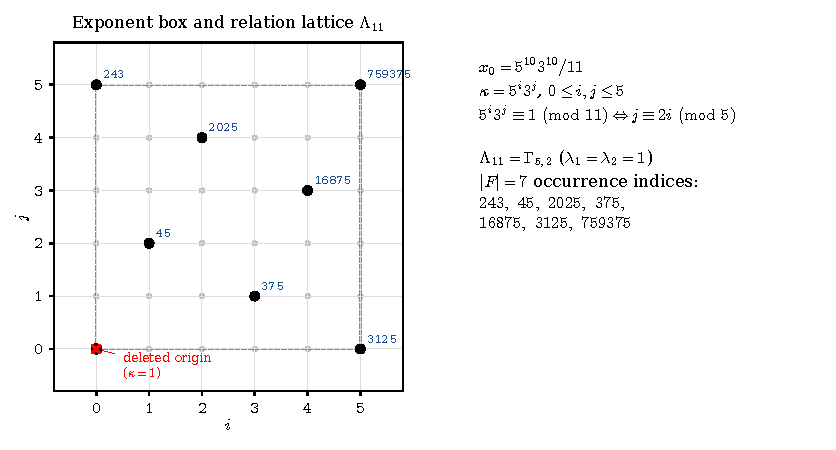
\includegraphics[width=\textwidth]{figures/fig01_fibre.pdf}
\caption{The actual occurrence fibre of $x_0=5^{10}3^{10}/11$ in prime-exponent coordinates $(i,j)$ for $5^i3^j$. Left: the box $[0,5]^2$, the lattice $\Lambda_{11}=\Gamma_{5,2}$ (black points; grey points are other integer points of the box), the deleted origin $\kappa=1$, and the occurrence indices $\kappa=5^i3^j$ at each point. Right: the defining congruence and the seven occurrence indices.}\label{fig:fibre}
\par\smallskip\noindent\figdesc{Seven black points at $(0,5),(1,2),(2,4),(3,1),(4,3),(5,0),(5,5)$ in the square $[0,5]^2$ with grey points at the remaining integer points; the origin is marked in red as deleted. Each black point carries its index $\kappa$ ($243$, $45$, $2025$, $375$, $16875$, $3125$, $759375$). The right panel states $5^i3^j\equiv1\pmod{11}\iff j\equiv2i\pmod5$.}
\end{figure}

%% -------------------------------------------------------------------
\section{Graver-cell geometry: definitions and elementary structure}\label{sec:cells}

From now on $d\ge2$ is an integer, $s\in\{1,\dots,d-1\}$ is a representative of a unit modulo $d$, $t\in\{1,\dots,d-1\}$ is the representative of $s^{-1}$, and
\[
  \Gamma=\Gamma_{d,s}=\{(i,j)\in\Z^2:\ j\equiv si\pmod d\}.
\]
Since $\Gamma$ is the kernel of the surjection $(i,j)\mapsto j-si\bmod d$, it is a sublattice of index $d$.

\begin{lemma}[Determinants]\label{lem:det}
For $g,h\in\Gamma$, $\cross(g,h)\equiv0\pmod d$.
\end{lemma}
\begin{proof}
Modulo $d$, $g_1h_2-g_2h_1\equiv g_1(sh_1)-(sg_1)h_1=0$.
\end{proof}

\subsection{Conformal order and Graver vectors}

\begin{definition}[Conformal order, Graver vectors]\label{def:conformal}
For $h,g\in\Z^2$ write $h\conf g$ if $h_ig_i\ge0$ and $|h_i|\le|g_i|$ for $i=1,2$. A nonzero $g\in\Gamma$ is a \emph{Graver vector} of $\Gamma$ if the only $h\in\Gamma$ with $h\conf g$ are $h=0$ and $h=g$. The set of Graver vectors is the \emph{Graver basis} $\mathcal G(\Gamma)$.
\end{definition}

The relation $\conf$ is a partial order on $\Z^2$ (reflexive, transitive, antisymmetric), and $\mathcal G(\Gamma)$ is the set of its minimal elements in $\Gamma\setminus\{0\}$. The Graver basis is symmetric: $g\in\mathcal G\iff-g\in\mathcal G$. For general lattices $\mathcal G$ is finite and contains every circuit; for $\Gamma_{d,s}$ we have the following explicit bound.

\begin{lemma}[Size of Graver vectors]\label{lem:graver-size}
Every Graver vector $g$ of $\Gamma$ satisfies $|g_1|\le d$ and $|g_2|\le d$. If $|g_1|=d$ or $|g_2|=d$ then $g\in\{\pm(d,0),\pm(0,d)\}$.
\end{lemma}
\begin{proof}
$(\pm d,0)$ and $(0,\pm d)$ lie in $\Gamma$ since $d\equiv0$. If $|g_1|\ge d$ then $h=(\mathrm{sgn}(g_1)d,0)\conf g$, $h\in\Gamma$, so by minimality $g=h$. If $|g_1|<d$ and $|g_2|\ge d$, symmetrically $g=(0,\pm d)$.
\end{proof}

\begin{lemma}[Standard Graver vectors]\label{lem:std-graver}
The following vectors are Graver vectors of $\Gamma_{d,s}$ (and so are their negatives):
\[
  (d,0),\quad (0,d),\quad (1,s),\quad (1,s-d),\quad (t,1),\quad (d-t,-1).
\]
\end{lemma}
\begin{proof}
$(d,0)$: if $h=(h_1,0)\conf(d,0)$ and $h\in\Gamma$, then $0\equiv sh_1$ forces $d\mid h_1$ because $s$ is a unit, so $h_1\in\{0,d\}$. The same for $(0,d)$ with the unit $s^{-1}$.

For the other four, let $g\in\Gamma$ have $|g_1|=1$ and $|g_2|<d$ (these are $(1,s)$ and $(1,s-d)$; their second coordinates satisfy $|s|,|s-d|<d$). If $h\in\Gamma$ with $h\conf g$, then $h_1\in\{0,g_1\}$. If $h_1=0$, then $d\mid h_2$ and $|h_2|\le|g_2|<d$, so $h=0$. If $h_1=g_1$, then $h_2\equiv sg_1\equiv g_2\pmod d$, $h_2$ has the sign of $g_2$ (or is zero) and $|h_2|\le|g_2|<d$; two integers congruent modulo $d$ of the same weak sign with absolute values below $d$ are equal, so $h=g$. The vectors $(t,1)$ and $(d-t,-1)$ are handled in the same way with the roles of the coordinates exchanged, using $t\equiv s^{-1}$: for $h\conf g$ with $|g_2|=1$, either $h_2=0$ and $d\mid h_1$ with $|h_1|\le|g_1|<d$, or $h_2=g_2$ and $h_1\equiv tg_2\equiv g_1\pmod d$ (indeed $sh_1\equiv g_2$ gives $h_1\equiv tg_2$, and $g_1\equiv tg_2$ for $g=(t,1)$ and $g=(d-t,-1)$).
\end{proof}

Lemma~\ref{lem:std-graver} proves the minimality of these six vectors without any box-dependent enumeration. It is the statement that supplies the Graver property of the generators $(1,-a)$ and $(c,-1)$, $a=d-s$, $c=d-t$, used for the bottom and left end cells in Section~\ref{sec:cellfamily}.

\subsection{Cells, the punctured fibre, and the realized union}

\begin{definition}[Punctured fibre and hull]\label{def:fibre}
For an integer box $Q=(Q_1,Q_2)$ with $Q_1,Q_2\ge0$ put
\[
  F_Q=F_{d,s,Q}=\bigl(\Gamma\cap[0,Q_1]\times[0,Q_2]\bigr)\setminus\{0\},\qquad H_Q=\conv(F_Q).
\]
\end{definition}

\begin{definition}[Admissible cells and the realized union]\label{def:cells}
Fix $Q$. An \emph{admissible parallelogram} is a set
\[
  P(w;g,h)=\conv\{w,\ w+g,\ w+h,\ w+g+h\}
  =\{w+\theta g+\eta h:\ \theta,\eta\in[0,1]\},
\]
where $g,h$ are linearly independent Graver vectors of $\Gamma$ and all four points $w,w+g,w+h,w+g+h$ lie in $F_Q$. An \emph{admissible segment} is $[p,p+g]$ with $g$ a Graver vector and $p,p+g\in F_Q$. An \emph{admissible point} is a point of $F_Q$. The \emph{realized union} $U_Q=U_{d,s,Q}$ is the union of all admissible parallelograms, admissible segments and admissible points.
\end{definition}

Every edge of an admissible parallelogram is an admissible segment, so the segments and points are needed only for boundary pieces and isolated points of $U_Q$ that are not contained in any parallelogram. Note that the same geometric parallelogram has several descriptions $P(w;g,h)$ (for example $P(w;g,h)=P(w+g;-g,h)$); we regard $P(w;g,h)$ as a subset of the plane, not as a triple.

\begin{figure}[ht]
\centering
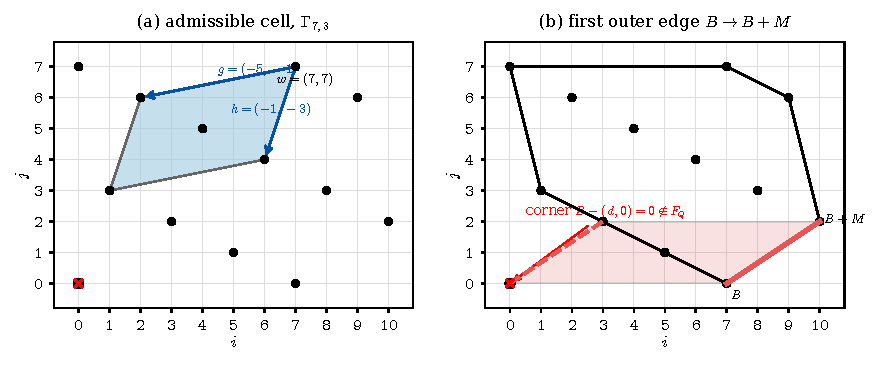
\includegraphics[width=\textwidth]{figures/fig02_cell.pdf}
\caption{(a) An admissible parallelogram $P(w;g,h)$ in $\Gamma_{7,3}$ with its two Graver generators $g,h$ and base point $w$ (the cell shown is the largest cell with corners in $F_{(7,7)}$). (b) The role of the deleted origin: the translate of the first outer edge $B\to B+M$ by $(-d,0)$ has the corner $B-(d,0)=0$, which is not in $F_Q$; this is why the first outer edge needs a separate cell (Section~\ref{sec:cellfamily}). Here $d=7$, $s=3$, $Q=(10,7)$.}\label{fig:cell}
\par\smallskip\noindent\figdesc{Left: grid of the box $[0,10]\times[0,7]$ with the lattice points of $\Gamma_{7,3}$ and one shaded parallelogram with two arrows labelled by its generators. Right: the same box, the convex hull of the points, the first edge leaving $B=(7,0)$ to the right drawn thick, and its translate by $(-7,0)$ drawn dashed with a red arrow to the origin, marked ``$B-(d,0)=0\notin F_Q$''.}
\end{figure}

\subsection{Elementary properties}

\begin{proposition}[Elementary properties]\label{prop:elem}
For every $Q\ge0$:
\begin{enumerate}
\item (\emph{Finiteness.}) There are finitely many admissible parallelograms, segments and points.
\item (\emph{Closedness.}) $U_Q$ is compact.
\item (\emph{Hull inclusion.}) $F_Q\subseteq U_Q\subseteq H_Q$.
\item (\emph{Monotonicity.}) If $Q\le Q'$ componentwise then every admissible cell for $Q$ is admissible for $Q'$ and $U_Q\subseteq U_{Q'}$.
\item (\emph{Transposition.}) Let $\tau(i,j)=(j,i)$. Then $\tau(\Gamma_{d,s})=\Gamma_{d,t}$ with $t\equiv s^{-1}$, $\tau$ preserves the conformal order, $\tau(F_{d,s,Q})=F_{d,t,(Q_2,Q_1)}$ and $\tau(U_{d,s,Q})=U_{d,t,(Q_2,Q_1)}$.
\item (\emph{Symmetry.}) The Graver basis is invariant under $g\mapsto-g$; $U_Q$ is unchanged if each cell $P(w;g,h)$ is described using $(-g,h)$ or $(g,-h)$ from the opposite corner.
\end{enumerate}
\end{proposition}
\begin{proof}
(1) Every cell is determined by its corner(s), which are points of the finite set $F_Q$ (the generators are differences of corners). (2) $U_Q$ is a finite union of compact convex sets. (3) $F_Q\subseteq U_Q$ by admissible points; each cell has its vertices in $F_Q\subseteq H_Q$, and $H_Q$ is convex, so $U_Q\subseteq H_Q$. (4) $F_Q\subseteq F_{Q'}$ and the Graver property is a property of $\Gamma$ only, not of $Q$. (5) $j\equiv si\iff i\equiv tj$; the map $\tau$ is a coordinate permutation, so it preserves $\conf$ and sends the box $[0,Q_1]\times[0,Q_2]$ to $[0,Q_2]\times[0,Q_1]$ and parallelograms to parallelograms. (6) Clear from $P(w;g,h)=P(w+g;-g,h)$.
\end{proof}

\begin{remark}
Items (1)--(4) are used silently throughout; (5) is the reason that proofs in Parts~II and III need to be carried out only for one of two symmetric configurations.
\end{remark}

\subsection{The abstract complex, the realized union, and an embedded subdivision}\label{sec:kabs}

The construction above admits three different mathematical readings which must not be confused.

\begin{definition}[$K_{\mathrm{abs}}$, $U_Q$, $K_{\mathrm{emb}}$]\label{def:kabs}
\begin{enumerate}
\item The \emph{abstract complex} $K_{\mathrm{abs}}(Q)$ is the finite regular cell complex whose vertices are the points of $F_Q$, whose edges are the admissible segments of dimension one, and whose $2$-cells are the distinct admissible parallelograms (as subsets of the plane), each attached along its four boundary edges. As a topological space it is the quotient of the disjoint union of its closed cells under the identification of shared faces by their vertex sets.
\item The \emph{realized union} is the subset $U_Q\subseteq\R^2$ of Definition~\ref{def:cells}. There is a natural continuous surjection $\pi:|K_{\mathrm{abs}}(Q)|\to U_Q$ which sends each cell affinely onto its geometric image.
\item An \emph{embedded subdivision} $K_{\mathrm{emb}}(Q)$ is any finite polyhedral complex in $\R^2$ with $|K_{\mathrm{emb}}|=U_Q$ in which every admissible cell is a union of cells; for instance the arrangement of all lines through all edges of cells, restricted to $U_Q$. It exists because $U_Q$ is a finite union of convex polygons, segments and points.
\end{enumerate}
\end{definition}

The map $\pi$ is a homeomorphism if and only if the relative interiors of distinct cells are pairwise disjoint and any two cells meet in a common face (compare the face-closed embeddedness criterion in the GEO-I record, listed in Appendix~\ref{app:registry} as context only). In general neither is true: distinct admissible parallelograms can overlap in a region, so that $\pi$ is not injective, and $|K_{\mathrm{abs}}|$ and $U_Q$ need not even have the same Betti numbers. The set $U_Q$ is a compact polyhedron regardless, and its topology is determined by $K_{\mathrm{emb}}$.

\begin{example}[Overlapping cells]\label{ex:overlap}
For $(d,s,Q)=(5,2,(5,5))$ there are exactly four distinct admissible parallelograms. With $v_1=(1,-3)$, $v_2=(2,-1)$, $f=(1,2)$,
\[
\begin{aligned}
C_1&=P\bigl((0,5);v_1,v_2\bigr), &C_2&=P\bigl((1,2);f,v_2\bigr),\\
C_3&=P\bigl((1,2);f,(3,1)\bigr), &C_4&=P\bigl((2,4);v_1,v_2\bigr).
\end{aligned}
\]
Each has area $5=d$, so the cells have total area $20$. The realized union $U_Q$ has area $17.5-5=12.5$ (Theorem~\ref{thm:exceptional}), so the total area of the cells exceeds the area of their union by $7.5$. The statements proved in this paper concern the set $U_Q$ and not $K_{\mathrm{abs}}$.
\end{example}

\begin{remark}[Modelling choice]\label{rem:modelling}
The attachment rule of Definition~\ref{def:cells} is a modelling decision. Arithmetic gives the lattice points (Theorem~\ref{thm:occ}) and the relations between them (Section~\ref{sec:arith-meaning}) exactly. Which one-dimensional and two-dimensional pieces to attach is a choice of geometry, made so that each attached piece is spanned by primitive relations among occurrence coordinates. A different attachment rule could yield different topology; it would not alter any statement about lattice points. Consequently, ``the topology of the occurrence fibre'' in this paper always means the topology of $U_Q$, as in the abstract.
\end{remark}

\begin{remark}[Convexity versus embedding]
Theorem~\ref{thm:universal} states $U_Q=H_Q$. It does not say that the admissible cells form a face-to-face tiling of $H_Q$, and in general they do not (Example~\ref{ex:overlap}, and the figures in Part~III in which cells of different colours overlap). The convex hull $H_Q$ itself is contractible, so a statement $U_Q=H_Q$ determines the topology of $U_Q$ without any information about $K_{\mathrm{abs}}$.
\end{remark}
